%%%%%%%%%%%%%%%%%%%%%%%%%%%%%%%%%%%%%%%%%%%%%%%%%%%
%% LaTeX book template                           %%
%% Author:  Amber Jain (http://amberj.devio.us/) %%
%% License: ISC license                          %%
%%%%%%%%%%%%%%%%%%%%%%%%%%%%%%%%%%%%%%%%%%%%%%%%%%%

\documentclass[a4paper,12pt,oneside]{book}
\usepackage[T1]{fontenc}
\usepackage[utf8]{inputenc}
\usepackage{lmodern}
%%%%%%%%%%%%%%%%%%%%%%%%%%%%%%%%%%%%%%%%%%%%%%%%%%%%%%%%%
% Source: http://en.wikibooks.org/wiki/LaTeX/Hyperlinks %
%%%%%%%%%%%%%%%%%%%%%%%%%%%%%%%%%%%%%%%%%%%%%%%%%%%%%%%%%
\usepackage{hyperref}
\usepackage{graphicx}
\usepackage[english]{babel}
\usepackage{titlepic}
\usepackage{wrapfig}

\graphicspath{{./images/}}
\setlength\parindent{0pt}
%%%%%%%%%%%%%%%%%%%%%%%%%%%%%%%%%%%%%%%%%%%%%%%%%%%
% First page of book which contains 'stuff' like: %
%  - Book title, subtitle                         %
%  - Book author name                             %
%%%%%%%%%%%%%%%%%%%%%%%%%%%%%%%%%%%%%%%%%%%%%%%%%%%

% Book's title and subtitle
\title{
	\Huge \textbf{Hybrid rendering}\\
	\huge using Radeon Rays
}
\titlepic{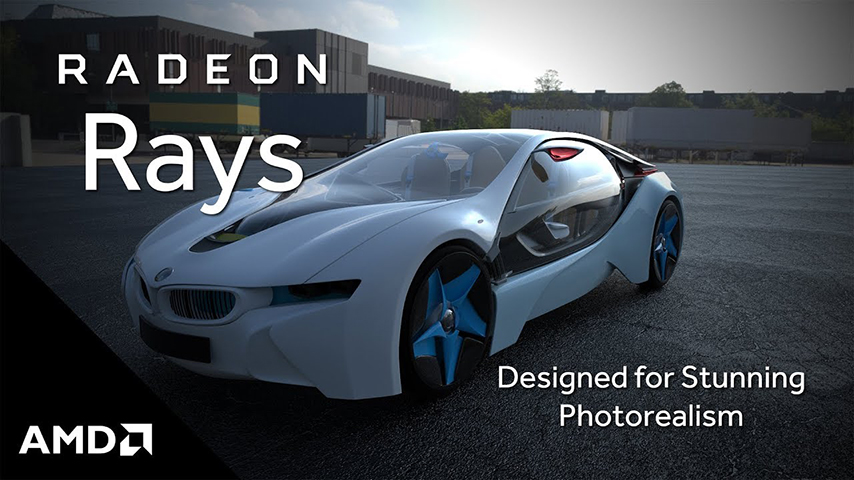
\includegraphics[width=\textwidth]{radeonrays.jpg}}
% Author
\author{
	Stijn Billiet\\\\
	Graduation work 2018-19\\
	Digital Arts And Entertainment\\
	howest.be
}
\date{}


\begin{document}

\frontmatter
\maketitle
\cleardoublepage
%%%%%%%%%%%%%%%%%%%%%%%%%%%%%%%%%%%%%%%%%%%%%%%%%%%%%%%%%%%%%%%%%%%%%%%%
% Auto-generated table of contents, list of figures and list of tables %
%%%%%%%%%%%%%%%%%%%%%%%%%%%%%%%%%%%%%%%%%%%%%%%%%%%%%%%%%%%%%%%%%%%%%%%%
\tableofcontents

\mainmatter
\chapter{Abstract}
This paper was written in an effort to elaborate on hybrid solutions between modern day rasterization engines and powerful ray-tracing ones and to explain rather thoroughly how one could implement this.

TODO methods
TODO results

\chapter{Introduction}
Ray-tracing is usually used in VFX productions to create the most accurate lighting effects, this doesn’t come for free though seeing crisp ray-traced images require countless hours of rendering. With the rise of new ray-tracing capable hardware (e.g. Volta architecture NVIDIA) things are about to change, developers are already putting ray-tracing in some parts of their pipelines, they must however rely on optimization (e.g. De-noising) to keep up with the performance demands. So for the time being we will see a lot of hybrid solutions, but we should see full ray traced engines by the time that our hardware is capable enough.\newline\par

That being said I would like to clarify that rasterization engines aren’t bad, however they are very rough approximations and rely on specific techniques to achieve lighting effects sometimes at the cost of artifacts. We must keep in mind though rasterization engines are here to stay for a while longer due to their immense performance, and not to forget they have been around for a while, their maturity surely pays off seeing what we’ve already achieved with rasterization (e.g. The Witcher 3: Wild Hunt).\newline\par

As the subtitle suggests we will use Radeon Rays for our ray-tracing algorithm, however there are other options out there like Microsoft's DirectX Raytracing. Nevertheless the topics outlined should still hold up when implementing an other API, only the Radeon Rays implementation details would be an exception to that rule. The same essentialy goes for our graphics card specification, OpenGL was used seeing that would be the logical combination, but the information should translate over nicely to other API's. \newline\par

%%%%%%%%%%%%%%%%
% NEW CHAPTER! %
%%%%%%%%%%%%%%%%
\chapter{Research}

This extract should give you a rather thorough overview of the technologies used, however some knowledge regarding graphics programming and/or matrix mathematics is advised.\newline\par

\section{Rendering techniques}
Over the past century many rendering algorithms have been researched/employed. They are all trying to find an answer to the problem of limited rendering capabilities. Seeing that our modern model of light would be completely impractical when it comes to (high speed) simulations, meaning it would take an obscene amount of time to calculate.\newline\par

Therefore people have come up with ways to more efficiently model the phenomenon of light. The most prominent models being: ray tracing (ray casting) and rasterization. The aforementioned models will be covered in the following subsections.

\pagebreak

\subsection{Raytracing}

\begin{figure}[h]
	\caption{Illustration of different ray-casting solutions}
	\centering
	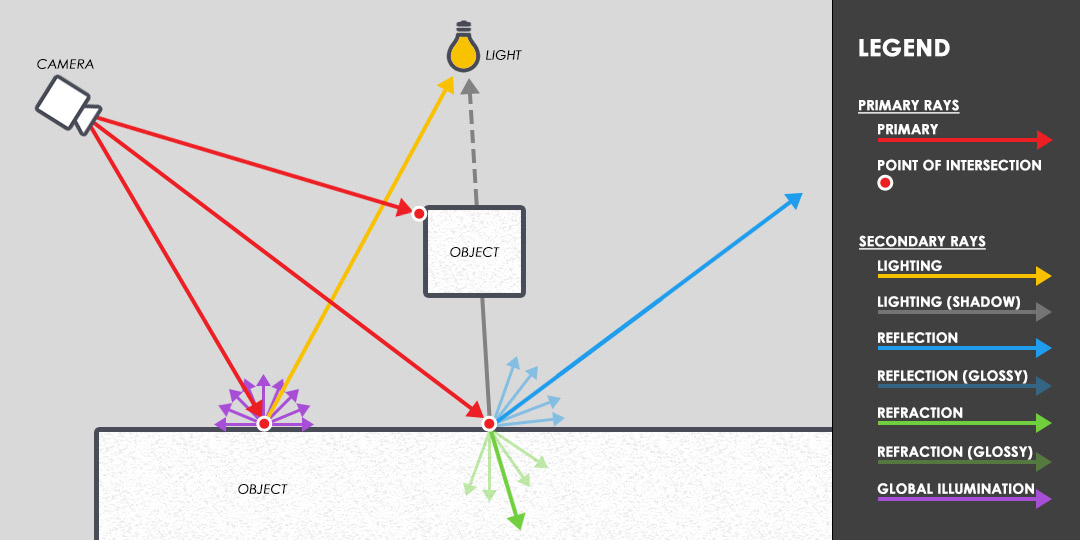
\includegraphics[width=0.95\textwidth]{raycasting.jpg}
\end{figure}
\subsubsection{Definition}
In short ray-tracing is a rendering technique that can produce lifelike lighting effects. A ray-tracing algorithm essentially achieves this by sending out rays for every pixel of our framebuffer (camera) towards the corresponding scene geometry. Based on the technique we can send out additional bounces (secondary rays). It then basically backtracks that chain of light-rays to accumulate material/light information to then calculate the final pixel color.

\subsubsection{Ray casting}

As addressed before ray-tracing essentially probes material and light information through the use of rays. There are 2 sets of rays, we've got primary rays and secondary rays. Primary rays are the first rays being sent out, the rays from camera towards the scene geometry. These primary rays are essentially doing the same as with rasterization in the sense that they only probe at material information. It becomes interesting however when we cast our secondary rays, these secondary rays have their origins at the interception point of the primary rays and the scene geometry. Their direction on the other hand are totally dependent on the technique that is employed, meaning that we will use different techniques to bounce/direct them based on the effect required  (e.g. shadows, reflections, etc.).\newline\par

\pagebreak

\subsection{Rasterization}

\begin{figure}[h]
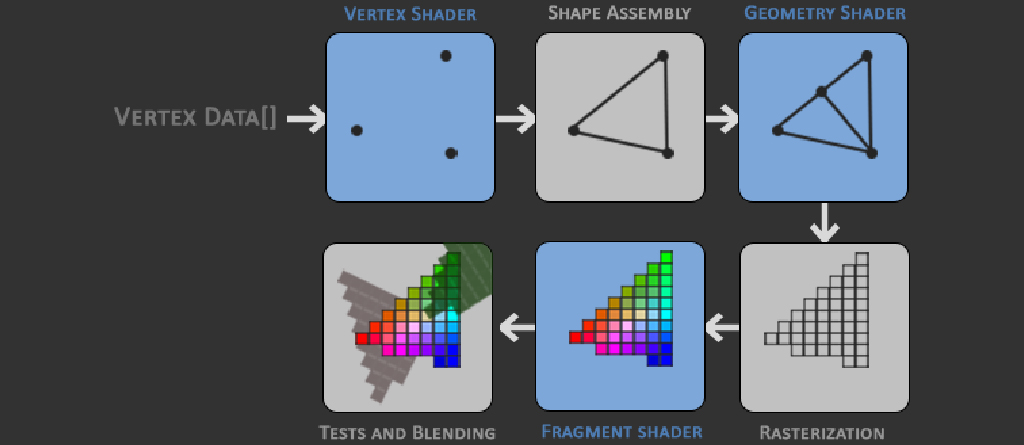
\includegraphics[width=\textwidth]{rasterization.jpg}
\caption{Rasterization graphics pipeline.}
\end{figure}

\subsubsection{Definition}
Rasterization is an algorithm designed to display three-dimensional objects on a two-dimensional screen. It's very fast seeing this algorithm is parallel in nature and can thus make full use of the GPU. The results of rasterization have gotten very good over the years, very convincing at relatively low compute performance. However there are certain limitations to this algorithm, seeing its main goal is to get graphics in screen space.\newline\par

\subsubsection{Graphics pipeline}
With rasterization objects on screen are created from meshes. A mesh is a collection of three-dimensional points a.k.a. vertices. These vertices are the main resource needed for rendering, these go through what's called the rendering pipeline to then be converted into screen pixels. The rendering pipeline or more formerly known as the graphics pipeline acts as a conceptual model that describes what steps a graphics system needs to performs to be able to render aforementioned meshes to a 2D screen. \newline\par
\pagebreak

\subsubsection{Vertex shader}
\begin{figure}[h]
	\centering
	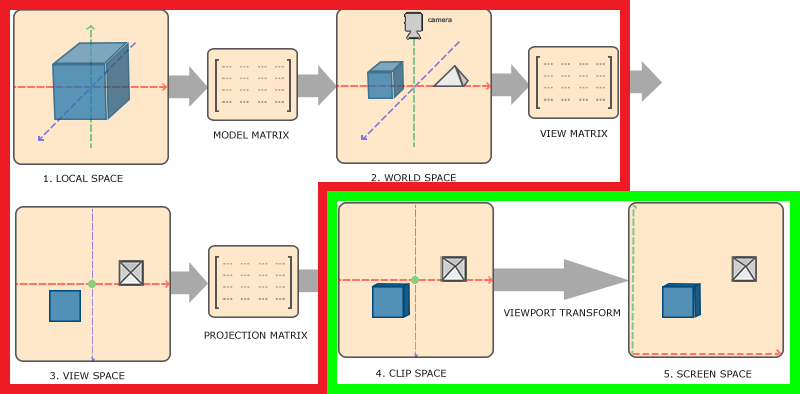
\includegraphics[width=0.8\textwidth]{coordinate_systems.png}
	\caption{Model space to screen space.}
	\label{fig:coordinates}
\end{figure}
The first stage is the vertex shader which essentially transforms the vertices to their correct
positions, the vertices have to be transformed seeing that they are defined in their own local transform space(vertices positions are defined relative to their own center point). The vertices are defined this way as a means to make it easier for modelers, they quite simply have to define the vertices relative to the modeling software's gizmo.

\subsubsection{Shape assembly}
\begin{figure}[h]
	\centering
	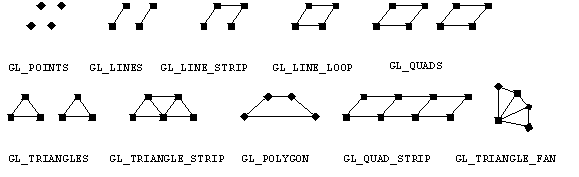
\includegraphics[width=\textwidth]{primitives.png}
	\caption{List of possible OpenGL primitives.}
\end{figure}

The second stage is the shape assembly which is in charge of creating primitives out of these verts. The developers have to specify the wanted primitive (e.g. triangle) the GPU then uses that information to interpret the a collection of vertices as said primitive.\newline\par

\pagebreak

\subsubsection{Geometry shader}
\begin{figure}[h]
	\centering
	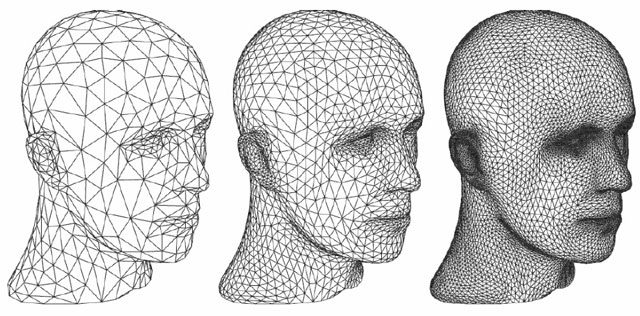
\includegraphics[width=0.7\textwidth]{geometryshader.jpg}
	\caption{Purpose of geometry shader.}
\end{figure}
The third stage is an optional geometry shader, this stage won't be covered in depth, but it is essentially in charge of creating additional geometry (extra vertices) at runtime.\newline\par

\subsubsection{Rasterization stage}
The fourth stage is rasterization, this is where the algorithm gets its name. The rasterizer is in charge of a not only rasterization, but also homogeneous divide, clipping, culling and viewport transform. \newline\par

\begin{minipage}{0.5\textwidth}
	\centering
	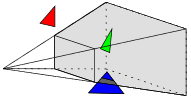
\includegraphics[width=\textwidth]{culling.png}
\end{minipage} \hfill
\begin{minipage}{0.5\textwidth}
	The first task of the rasterizer is primitive culling. The shapes that made it to the rasterizer are checked based on their normals. The normal of a primitive/vertex tells us if the face is facing away from us or not. This simple operation can be demonstrated using the dotproduct, however this does get handled by the specifications (e.g. DirectX/OpenGL) rasterizer. In its essence the calculation will translate to if the dotproduct is negative then the face is facing away, if it's positive then it's facing toward us.
\end{minipage}

\pagebreak

\begin{minipage}{0.5\textwidth}
	The second task is the clipping stage, in this stage we clip triangles that lie (partly) outside of the view frustum. This effectively removes those triangles and prevents them from being projected/rendered. 
\end{minipage} \hfill
\begin{minipage}{0.5\textwidth}
	\centering
	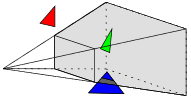
\includegraphics[width=0.8\textwidth]{clipping.png}
\end{minipage}

\vspace{0.5cm}

\begin{minipage}{0.4\textwidth}
	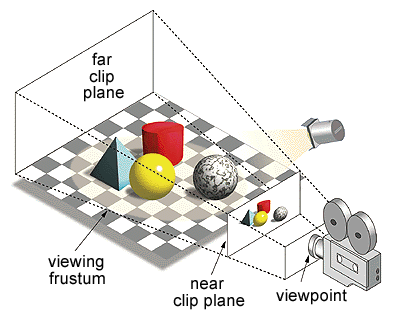
\includegraphics[width=\textwidth]{frustrum.png}
\end{minipage} \hfill
\begin{minipage}{0.59\textwidth}
	The third task of the rasterizer is the homogeneous divide. The previous stages were in charge of transforming the vertices from model space into clipping space, this is done by multiplying the world, view and projection matrix with the vertices this yields a valid projection but does not account for depth information (f.e. objects that are nearby will appear the same as objects from afar) this is where the z-component comes in, seeing the z stores our depth information. Before we apply the projectionmatrix we store the z-component as an additional w component.
\end{minipage}

\vspace{0.25cm}

The homogeneous divide is just a specific term for converting the homogeneous coordinate back to w=1 meaning we put the vertices in their normalized device coordinates (in the -1 to 1 range) effectively scaling all objects to their rightful dimensions.\newline\par

The fourth stage is the viewport transform. In the viewport transform we essentially translate all the vertex positions that are now in normalized device coordinates (NDC) and transform them to window space. These are then the coordinates that are being rasterized to the output image. This process is outlined in figure \ref{fig:coordinates} (part with green outline).

\vspace{0.5cm}

\begin{minipage}{0.55\textwidth}
	The final task pixelisation (rasterisation) is the process of converting continuous primitives into discrete pixel fragments. The rasterizer does so by interpolating between vertex attributes (data that vertex holds) like color, normals, texture coordinates and positions. It then launches a fragment shader for every pixel fragment with the information just calculated.
\end{minipage} \hfill
\begin{minipage}{0.4\textwidth}
	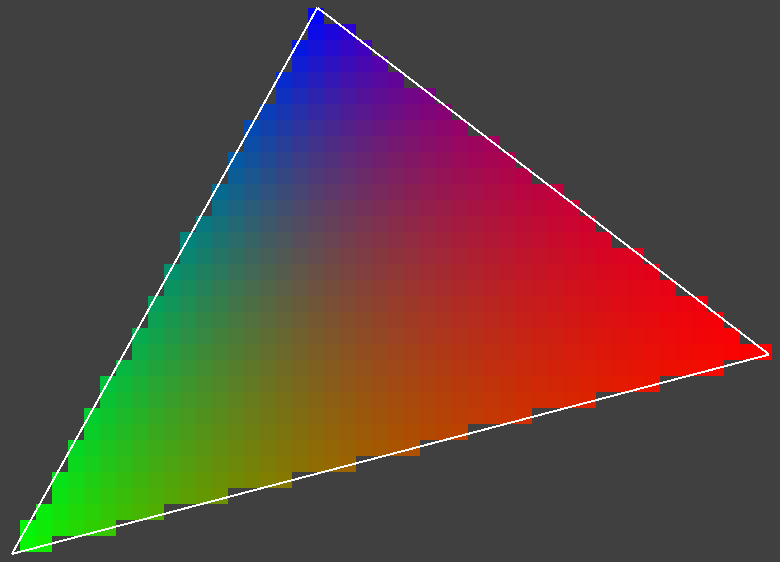
\includegraphics[width=0.95\textwidth]{pixelisation.png}
\end{minipage}

\pagebreak

\subsubsection{Fragment shader}

\begin{figure}[h]
	\centering
	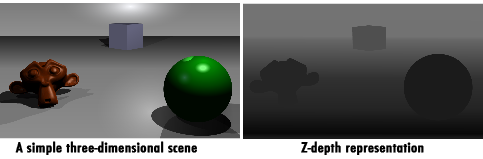
\includegraphics[width=0.85\textwidth]{Zbuffer.png}
\end{figure}
The fifth stage, the fragment stage is a shader stage that will process all pixel fragments processed by the rasterizer. Depending on the technique we collapse all information into a set of colors (color buffer) and a single depth value (depth buffer), additionally we can augment this by writing away a stencil value (stencil buffer).

\subsubsection{Test and blending stage}
\begin{figure}[h]
	\centering
	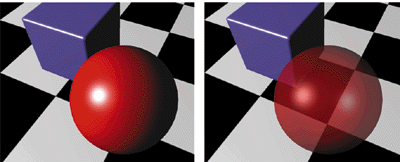
\includegraphics[width=0.8\textwidth]{alpha.png}
\end{figure}
Finally we've got the testing and blending stage. Up until this point "pixels" where addressed as pixel fragments, this is in-fact a clear distinction to make seeing that pixel fragments are not guaranteed to show up on screen, they could be discarded in the shaders or they could be transparent. If there are transparent objects in the scene we have to keep both pixels, those from the object behind it and the transparent object, we can then simply blend those pixels together to receive the final pixel colour. This blending operation is in-fact quite costly seeing we need to make sure the objects appear in the right order and we've got the load of additional pixels on our hands. A more optimized technique can be used for objects that are fully transparent however, here we can employ alpha testing where we simply discard those pixel fragments in the fragment shader.

\pagebreak

\section{API's and tools}

The main API's that have been researched were Radeon Rays, OpenCL and OpenGL. However to speed up the development process tools were employed. The main part of the tools were tailored towards the OpenGL pipeline (e.g. model loading, texture loading, etc.), but some small frameworks were also employed to speed up the raytracer development (e.g. CLW). Keep in mind however that these tools are not necessary seeing it could all be made on your own, but it sure helps to have these around.

\subsection{Raytracing}
\subsubsection{OpenCL}
Open Computing Language is a framework for writing programs that execute across compute devices. This includes among other hardware accelerators, the central processing unit (CPU) and the graphics processing unit (GPU). These aforementioned programs are called kernels and are also written on a pseudo c-language. OpenCL provides the programmer of a standard interface to perform parallel computing tasks. The programmer has to set up the OpenCL execution pipeline and write the kernels.

\begin{figure}[h]
	\centering
	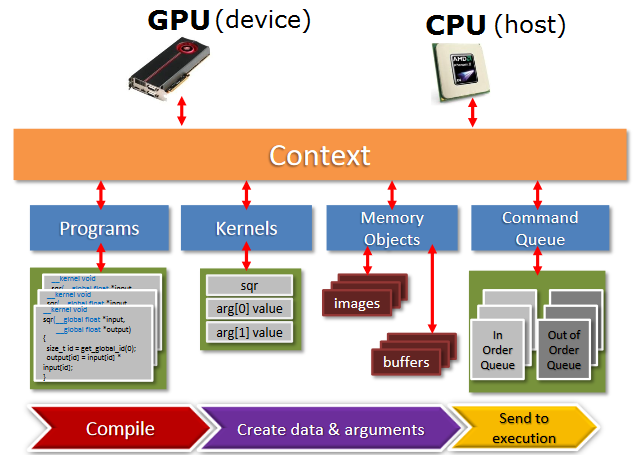
\includegraphics[width=0.9\textwidth]{openclprogram.png}
\end{figure}
Under this section you'll find a quick rundown of aforementioned execution 
model.
\pagebreak
\begin{itemize}
	\item{\textbf{Platform}}\newline\par
	The platform that we are running this code on, so which vendor (e.g. Nvidia).
	\item{\textbf{Device}}\newline\par
	What device are we going to run this on could be anything from CPU, GPU to APU.
	\item{\textbf{Context}}\newline\par
	This is the runtime interface between the host program (run on the CPU) and the device (CPU/GPU/etc.). The context is in charge of managing all the OpenCL resources so programs, kernels, command queues and buffers.
	\item{\textbf{Program}}\newline\par
	The entire OpenCL program, this could be one or more kernels/device functions bundled together into a single program file.
	\item{\textbf{Kernel}}\newline\par
	The starting point/building blocks of a OpenCL program. Kernels are called from the CPU, they provide the basic units of executable code that run on a OpenCL device. The kernels are preceded with the keyword "\_\_kernel"
	\item{\textbf{Command queue}}\newline\par
	The command queue allows the kernels execution commands to be sent to the device. This effectively queues them for execution, this en-queuing can be in-order or out-of-order.
	\item{\textbf{Memory objects}}\newline\par
	The memory objects are what is provided to the kernels. Kernels do accept basic types like floats, ints, bools etc. and self defined types like Ray, Intersection etc, but if there is a large buffer of those it's kept in a Memory buffer (e.g. images).
\end{itemize}

A large part of the parallelization control is in the hands of the programmer. Upon launching a kernel the programmer is in control of how many work items need to be handled per compute unit, this effectively bundles them in a workgroup. Each workgroup gets its own compute unit, a work group can exist out of one or multiple work items. This degree of freedom is further reinforced by the level of control over different memory levels that can be employed to speed up development.\newline\par

\begin{figure}[h]
	\centering
	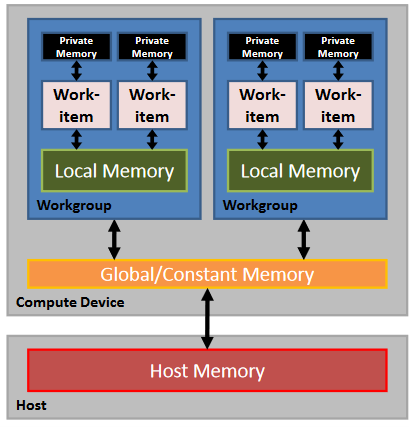
\includegraphics[width=0.7\textwidth]{memorymodel.png}
	\caption{Illustration of the memory execution model.}
\end{figure}

Under this section is a roundup of the OpenCL memory model (GPU memory model).\newline\par
\pagebreak

\begin{itemize}
	\item{\textbf{Global memory}}\newline\par
	Global memory is very similar to RAM, it is the largest memory buffer but also the slowest. Global memory can be written to / read from by all work items (or threads).
	\item{\textbf{Constant memory}}\newline\par
	A small chunk of global memory on the device, can be read from by all work items, but can not be written to. However the host application has full read/write access to this memory pool. Constant memory is a bit faster than 
	\item{\textbf{Local memory}}\newline\par
	The local memory is a shared memory pool among work items in the same work group, similar to cache on the CPU. Local memory allows work items to share their results with work items belonging in the same work group. Local memory is up to 100 times faster than global memory.
	\item{\textbf{Private memory}}\newline\par
	The fastest type of memory, similar to registers on the cpu. Each work item (thread) has a tiny buffer of private memory to store intermediate results in.
\end{itemize}

\pagebreak

\begin{figure}[h]
	\centering
	\includegraphics[width=\textwidth]{sharegroups.png}
	\caption{OpenCL/OpenGL interop context}
\end{figure}

A great thing about this control over memory is that it empowers the developer to make use of interoperation contexts. This can be used to achieve zero-copy architectures where memory objects can be shared by multiple compatible api's. A prime example of this is an OpenCL/OpenGL interop context. Such a context allows the graphics programmers to send screen buffers, textures and openGL objects to the kernels for further processing without the need to copy them, further enabling them to use a kernel in the pipeline everywhere they want.\newline\par

While this is great, there are still some limitations that have to be set in place to enable this kind of behaviour. For one the target device needs to support this sharegroup behaviour and for seconds shared memory can cause issues seeing that both contexts don't know about each others existance. All of this can be alliviated by setting blocking calls (e.g. GPU fences) in place, with these acting as a sort of failsafe that makes sure the object is done reading from/ writing to by the target context. This can account for slowdowns seeing that the CPU is needed to help the 2 parties synchronize, luckily for the programmer there is hope that said GPU supports the ARB\_cl\_event extension.3 The event extension allows the two api's to communicate through event management (e.g. wait for event to begin) ensuring that they don't need to wait a few ticks of CPU-time to synchronize.

\pagebreak

\subsubsection{Radeon Rays}
Radeon-Rays is a GPU intersection library(raytracing framework), was developed by AMD and it is featured in their AMD ProRenderer (raytraced renderer).
Radeon Rays exposes a well defined C++ API for scene construction and performing asynchronous ray intersection queries.\newline\par
Radeon-Rays employs OpenCL kernels to do all these calculations and to speed up the ray intersection they order their objects in bounding volume hierarchies. Seeing they use OpenCL to speed up their computations by sending it of to the GPU, this library will run on almost any GPU (meaning it will also work on Nvidia/Intel products).

\subsection{Rasterization}
\subsubsection{OpenGL}
\begin{itemize}
	\item{\textbf{OpenGL}}
	\pagebreak
	\item{\textbf{Loading libraries}}\newline\par
	OpenGL is a specification that has many different versions, implementations and features. The hardware manufacturers have to make sure their hardware/drivers provides the graphics programmers of those features. However when working with immensely different target platforms, ranging from old hardware to new and from obscure cards to bleeding edge ones the graphics programmers need some kind of way to determine what's possible on that specific piece of hardware. That is where loading libraries come in, loading libraries essentially provide the programmer with function pointers to OpenGL agnostic functions at runtime, meaning they provide us the memory addresses of those functions seeing they depend from hardware to hardware.\newline\par
	
	An additional task of the loading libraries is extension loading where programmers can use this API to ask if a specific extension/feature is supported on the hardware. Loading libraries provide their own OpenGL implementations (e.g. 'gl.h'), but your own implementation can be provided by making sure it is set as the last include in your build order. A word of caution however is that some features might be declared in your specification that the loading library has no knowledge of, but this is an edge case seeing that most people won't thread that route.\newline\par
	
	There are numerous libraries out there that do just that, libraries like GLEW, GL3W, Glad, Glee and many more. All libraries that exist out there all deliver on the same promise, meaning that the choice of library really boils down to personal preference.\newline\par
	\item{\textbf{GLM}}\newline\par
	When it comes to math libraries that plug in nicely with an OpenGL renderer there's really only one good option namely GLM. OpenGL Mathematics (GLM) is a header only C++ mathematics library for graphics software based on the OpenGL Shading Language (GLSL). \newline\par
	GLM exposes a well defined interface for everything from calculus to quaternion rotations (e.g. vector operations, matrix calculations).
\end{itemize}
\subsubsection{Window creation}
A window allows the rendering specification to offload its framebuffer to the viewport, it also acts as a layer between the operating system and the game when it comes to input etc. The creation of a window is entirely dependent on the operating system it's creating the window for. For example when creating a window on linux the X window system should be addressed, whereas on Windows you would need to hook on to the WinMain function and use the WndProc callback to fetch any input. Therefore it is much smarter to use a library that hides all this operating system agnostic stuff in an abstraction layer.\newline\par
SDL, SFML and GLFW are all low level libraries that handle multimedia indirection. They all deliver the same features in some shape or form. The choice really boils down to maturity of the library, documentation, usefulness of its features and frequency of the updates (if any).
\subsubsection{Texture loading}
A texture is a 2D (could be 3D or 1D) image packed with color data that is used to feed into the graphics pipeline to texturize geometry. Textures can be stored in a dozen of file formats, each with their own structure to store the pixel data. Textures are stored in a binary format and can therefore be parsed by a binary reader. The problem however with doing textureloading is that every format is different so the programmer would be in charge of writing a dozen different loaders to support the most basic of texture types. Seeing that this is rather cumbersome most people would opt for a library that does this for them. Again there are quite a lot of libraries out there that do this. \newline\par

SOIL, GLi, DevIL, FreeImage and stb\_image are all texture loading libraries that promise on loading the most prevalent of types.
\pagebreak

\subsubsection{Model loading}
\begin{itemize}
	\item{\textbf{3D file format}}\newline\par
	A 3D file format is a specification to store information about 3D models in the form of plain text or as binary data. The main purpose of such format is to encode 3D model's geometry, material information and animation data. Seeing there are loads of formats out there, creating your own model loading library has become something of a novelty. Fortunately there are loads of libraries out there that load about any format you throw at it.
	\item{\textbf{AssImp}}\newline
	
	\begin{figure}[h]
		\centering
		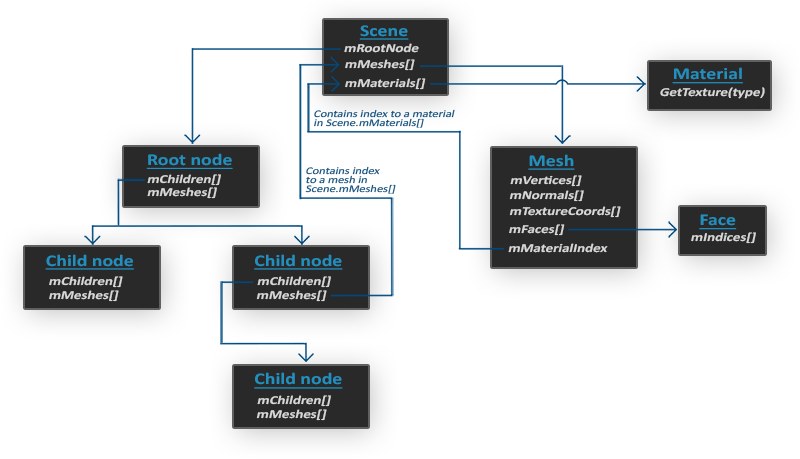
\includegraphics[width=0.9\textwidth]{assimpstructure.png}
	\end{figure}
	
	Asset import or AssImp for short is a model loading library designed to load as many formats as possible and to unify them into a searchable structure to be used by the host application. It structures the entire scene into a scene object, which consecutively holds a rootnode and a collection of meshes and materials. That rootnote then has leads to other nodes that all hold the same information namely a list of indices to the corresponding meshes and a next connection. This leads to a clear distinction as to what are seperate objects in the global model file, which can then later be used by the game-engine to ensure perfect relationships between aforementioned meshes.
\end{itemize}

\pagebreak

\section{Hybrid rendering approach}
The different rendering techniques have been covered, now onto a hybrid solution where rasterization and raytracing are combined to achieve a new pipeline. Most hybrid approaches replace the first stage of ray-tracing, which is sending out our primary rays to retrieve surface information, by rasterization. This effectively reduces the amount of rays by half. Ray-tracing comes into play for sending out our reflected rays, which could be anything from sending out new primary rays to secondary (shadow) rays. This introduction of ray-tracing essentially brings us world information whereas normally you'd only have surface information. To be able to augment rasterization with raytracing we will need to postpone our lighting effects to a later stage.

\subsection{Raytracing in rasterization}

\subsubsection{Forward vs deferred rendering}

\begin{figure}[h]
	\centering
	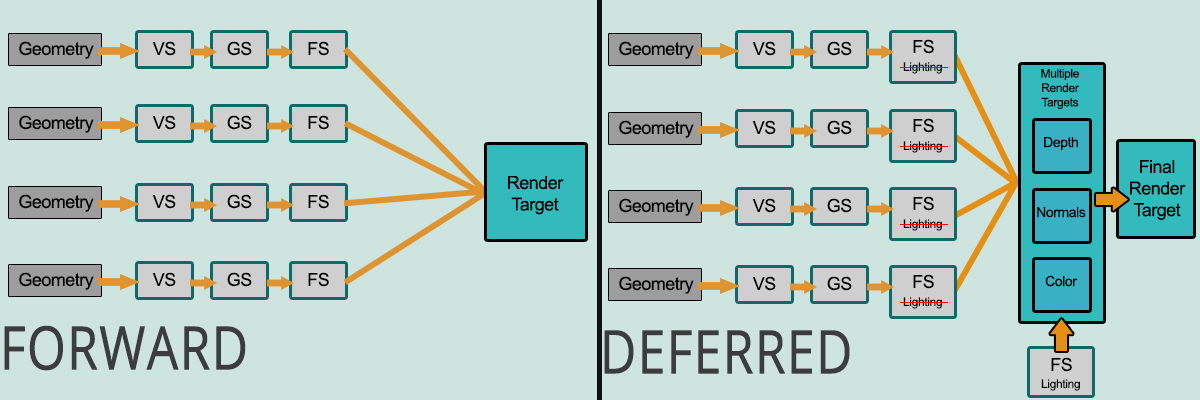
\includegraphics[width=\textwidth]{fvsdef.png}
	\caption{Difference between forward and deferred pipeline.}
\end{figure}

In rasterization there are three main lighting pipelines. The default pipeline is forward rendering this is the pipeline that's discussed in the previous chapters. The main difference between both pipelines however is in the way they handle the lighting effects. In forward rendering the lighting is applied per object in the fragment shader, this means that even the transparent objects, whose pixel fragments are not sure to end up in the final image, are also being handled. This pipeline is fine for default drawing, but starts to fall behind when it comes to lighting performance.\newline\par

\pagebreak

\begin{figure}[h]
	\centering
	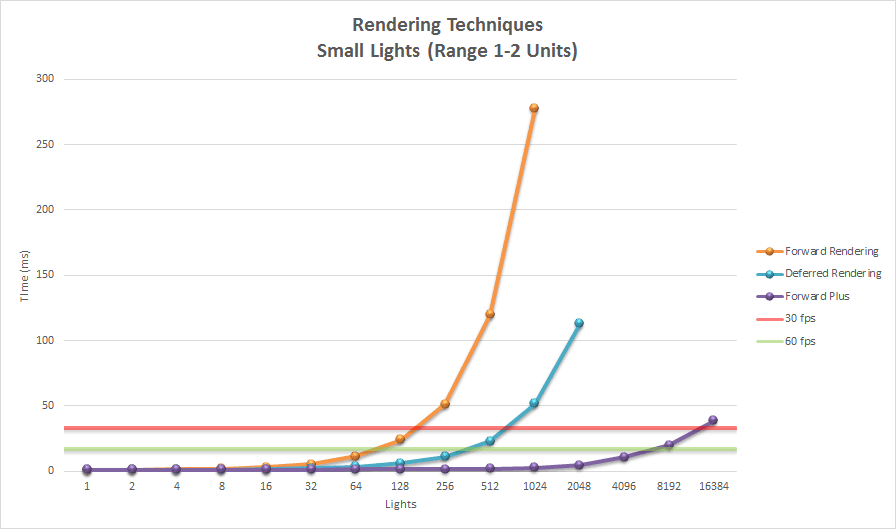
\includegraphics[width=\textwidth]{fvsdefgraph.png}
	\caption{Lighting performance comparison between forward and deferred.}
\end{figure}

The second pipeline however as the name suggests defers from doing any lighting effects until all the objects are rendered in the off-screen g-buffers. This effectively divides the pipeline into two major parts, the fill pass and the lighting pass. In the fill pass we fill up all the off-screen buffers (or G-Buffers) with our pixel in formation. The light pass as the name suggests is then in charge of applying lighting to those pixels. This ensures that we can postpone our lighting to the lightpass enabling us to do additional effects that encompass the whole scene (e.g. raytracing.)\newline\par

The third rendering pipeline, although the most performant will not be covered with explicit detail. The reason that this technique is not that applicable has primarily to do with the fact that we have no way of doing world space lighting effects. Forward+ is a rendering technique that improves upon regular forward rendering. Forward+ first determines which lights are overlapping which areas of the screen (screen space). During the shading phase that list is then consulted to only account for the lights that are potentially overlapping the current pixel fragment. The forward+ technique consists primarily of three simple passes. In the light culling pass, each light in the scene is sorted into screen space tiles. In the opaque pass, the light list generated from the light culling pass is used to compute the lighting for opaque geometry. The transparent pass is similar to the opaque pass in the sense that the light list is again consulted when shading the transparent pixel fragments.

\pagebreak

\subsubsection{Raytracing using g-buffers}

\begin{figure}[h]
	\centering
	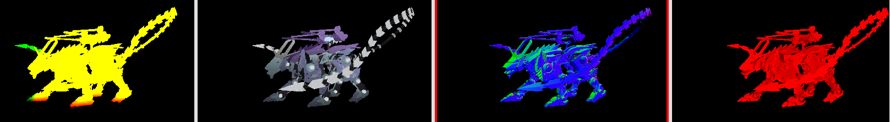
\includegraphics[width=\textwidth]{gbuffer.png}
	\caption{Illustration of g-buffers}
\end{figure}

As touched earlier deferred rendering fills the off screen render buffers (g-buffers) with scene information in its first pass. This effectively enables us to do lighting after the fact by then using that information to construct everything we need to apply our lighting.\newline\par

The information that is stored in the g-buffers is entirely up to the programmer (e.g. position data, normal data, color data etc.). However to be able to use this in conjunction with ray construction the programmer needs atleast the position data and the normal data. Some people would however argue that the position data isn't necessary and that the position can be calculated by the z-buffer and that would be an entirely correct answer, but for simplicity sake people opt for the position data instead.\newline\par

With the geometry data now in the g-buffers, that data can now be used to construct the rays. The ray construction can be sped up by doing it on the GPU, seeing that this operation is highly parallel in nature. Essentially what it boils down to is to make sure that meshes have been synchronized with the raytracer, meaning that the raytracer has all the right meshes in its scene to be able to fetch all occlusion/intersections. Then quite simply sample all the position entries and normal entries (for the entire screen) and send out a ray for every pixel, this will in turn correlate to the raytracer api seeing those position entries should correspond with the meshes in the scene.\newline\par

Once the rays have been constructed the raytracer can now simply query the occlusion/intersections with the scene geometry. That data can then be used to shade the object respectively.\newline\par

\pagebreak

%%%%%%%%%%%%%%%%
% NEW CHAPTER! %
%%%%%%%%%%%%%%%%
\chapter{Case study}
In the following chapter an example rendering pipeline will be covered. This pipeline will make use of deferred shading (rasterization) for its main pipeline and raytracing for real-time shadows. The implementation of the shadows acts as an example effect to display that there is gain to be had when replacing that with a raytraced counterpart. The case study will act as a logical guide on how to implement this pipeline yourself, but some situation agnostic details will be left open for interpretation.\newline\par

\section{Getting started}
\subsection{Building using CMake}

\pagebreak

\section{Implementation rasterization}
\subsection{Window creation}
\begin{figure}[h]
	\centering
	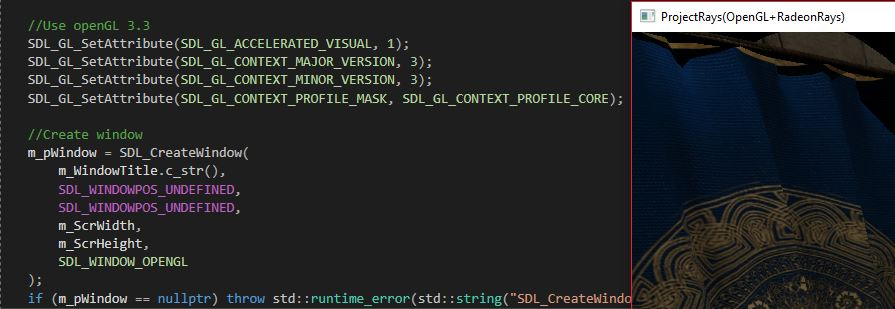
\includegraphics[width=\textwidth]{window.jpg}
	\caption{Snippet for window creation}
\end{figure}

The first main part that needs to be implemented to render is a window. As already outlined in the research part there are a lot of libraries out there. For this implementation SDL was chosen, simply for the reason that creating an SDL windowing context with OpenGL is a breeze. SDL expects the programmer to supply what version of OpenGL will be coupled to this window, what rendering mode will be used (e.g. immediate vs core) and the settings of the window. In our case we'll use OpenGL 3.3 seeing it was the first modern implementation of SDL and consecutively the easiest to comprehend, we'll also be using core mode seeing we need vertex buffer abilities.\newline\par

\subsection{Rendering specification}
\subsubsection{OpenGL function bindings}
Once the window and accompanying context is in place the programmer can move on to the OpenGL loading. For this implementation Glad was used. To get glad to work in this solution the respective package has to be created from their website \href{https://glad.dav1d.de/}. For our purpose I selected the GL 3.3 package in core functionality mode. After the package selection has been done you should receive the source files. These can then be compiled into a solution by making use of CMake, to then consecutively build those into lib files. The final step was to link both the includes and libs into my solution. A simple call to gladLoadGLLoader(SDL\_GL\_GetProcAddress) later and it's done.\newline\par

\pagebreak
\subsection{Shader loading}

\begin{figure}[h]
	\centering
	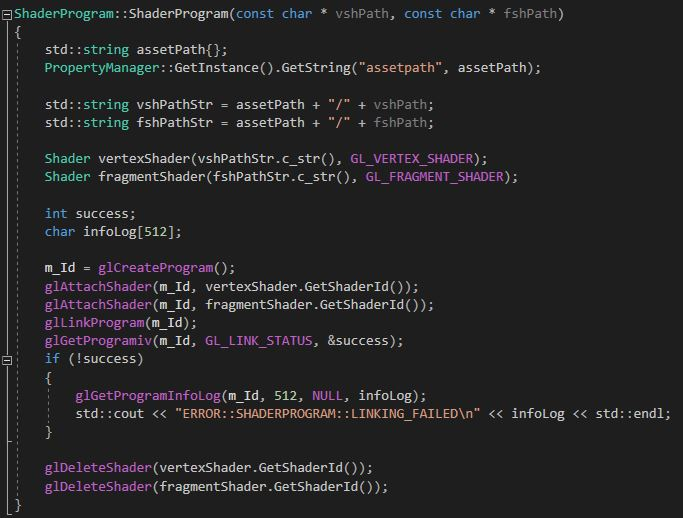
\includegraphics[width=\textwidth]{shader.jpg}
\end{figure}

One of the major things that make the graphics pipeline modular is programmable shaders. Shaders are mostly written in a pseudo c-language like GLSL/HLSL. This language is relative to the underlying rendering api that is being used. The rendering api is therefore in charge for the shader compilation. The only obstacle that the host program has to overcome is loading the source from the shader file. In this implementation the default cpp iostream was used, but this can be tailored to the needs of your engine/implementation. Once the shader source has been loaded it needs to be compiled and hooked to an OpenGL object. In this implementation a clear distinction between a shader and a shader program was made, where a shader is seen as the smallest building block and a shader program as a collection of those blocks.\newline\par

\subsection{Model loading}

\subsection{Texture loading}

\subsection{Coordinate systems}
Although you can render without a proper coordinate system in place, the implementation needed world space coordinates rather than screen space. \newline\par
So for this implementation a transform component was set in place. This transform component stands in relationship with the GameObject. This relationship allows us to add childs to the GameObject while maintaining the correct local transforms in the component. If the position of a said object was changed we go ahead and rebuild our worldmatrix while keeping in check if the object had a parent.\newline\par
The next part is the camera component, the camera component is in charge of holding the viewprojectionmatrix. Meaning that it is also in charge of holding the camera position and its settings.\newline\par
The final part to the puzzle is the mesh draw component. To create a meshdrawcomponent the programmer has to provide it with a mesh filter which is loaded by the model loading utilities mentioned prior. Then the final assembly is to build the worldviewprojectionmatrix (by multiplying the world, view and projection matrices with each other) and send it to the shader.

\subsection{Deferred shading}

\section{Implementation ray-tracing}

\subsection{OpenCL implementation}

\subsection{Radeon rays implementation}

\subsection{Shadow implementation}

\chapter{Conclusion}

\bibliographystyle{}
\bibliography{}
\begin{thebibliography}{Xyz12}
	
	\bibitem{voica14}
	Alexandru Voica,
	2014,
	Practical techniques for ray tracing in games,
	\url{http://www.gamasutra.com/blogs/AlexandruVoica/20140318/213148/Practical_techniques_for_ray_tracing_in_games.php}
	
	\bibitem{voica15}
	Alexandru Voica,
	2015,
	Ray tracing made easy,
	\url{http://www.alexvoica.com/ray-tracing-made-easy/#sthash.q1sHqqiT.dpbs}
	
	\bibitem{einig17}
	Mathieu Einig,
	2017,
	Hybrid rendering for real-time lighting: ray tracing vs rasterization,
	\url{https://www.imgtec.com/blog/hybrid-rendering-for-real-time-lighting/}
	
	\bibitem{caulfield18}
	Brian Caulfield,
	2018,
	What's the difference between ray tracing and rasterization?,
	\url{https://blogs.nvidia.com/blog/2018/03/19/whats-difference-between-ray-tracing-rasterization/}
	
	\bibitem{pipeline18}
	Wikipedia,
	2018,
	Graphics pipeline,
	\url{https://en.wikipedia.org/wiki/Graphics_pipeline}
	
	\bibitem{scratchapixel18}
	Scratchapixel,
	2018,
	Ray-Tracing: Generating Camera Rays,
	\url{https://www.scratchapixel.com/lessons/3d-basic-rendering/ray-tracing-generating-camera-rays}
\end{thebibliography}

%%%%%%%%%%%%%%%%
% NEW CHAPTER! %
%%%%%%%%%%%%%%%%
\chapter*{Appendices}

\end{document}
